\documentclass[a4paper]{article}

\usepackage{graphicx}
\usepackage[margin=3cm,noheadfoot]{geometry}

\begin{document}

\section{Epipolar geometry}
\label{epipolar}

\begin{figure}[h!]
  \label{fig:epipole}
  \centering
  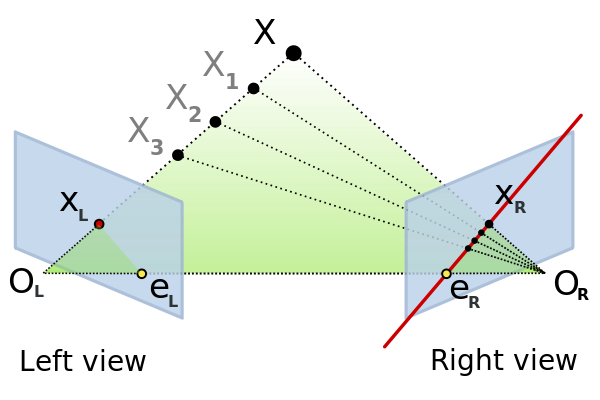
\includegraphics[width=1.0\textwidth]{Epipolar_geometry}
  \caption{All points $X_{1}, X_{2}, \cdots, X_{L}$ lie on the same epipolar line in the right view}
\end{figure}

Epipolar geometry is used in stereo vision to limit the searching space when
looking for matching points in both images. A point $X$ in 3D space is seen in
image $A$ as a point $x$, which is on the line between camera $A$'s focal point
and point $X$. This line is seen by camera $B$ as a line. This is called an
\emph{epipolar line}. Given both the cameras internal and external matrices and
a point $x_A$ we can generate an epipolar line corresponding to this point in
image $B$. This constrains the search space to this 1D line.

The points called $e_{L}$ and $e_{R}$ in figure \ref{fig:epipole} are called the
\emph{epipolar points} of both images. Epipolar lines rotate around the epipolar
point of a given image.

\section{Rectification}
\label{rectification}
As we have seen in section \ref{epipolar}, we can constrain the search space to
a 1D line. However due to the nature computers store images, it would be very
convenient if these epipolar lines were parallel to the horizontal scanlines.
This is done by a process called \emph{rectification}. This process transforms
both images so that the epipolar lines of the images align horizontally. For
this, we need a matrix that relates the two cameras. This matrix is called the
\emph{fundamental matrix} or \emph{bifocal tensor} and is denoted by the symbol
$F$.

\subsection{Fundamental matrix}
Given a point $x$ in image $A$, $Fx$ describes the epipolar line in image
$B$ on which the corresponding point $x'$ must lie. This means that $F$ has to
satisfy the equation
\[ x'^{T}Fx = 0 \]
for all corresponding points $x$ and $x'$. Given enough corresponding points, we
can solve this equation linearly. The more points available, the more accurate
this fundamental matrix becomes.\footnote{That is, if the corresponding points
are accurate as well.}

\subsection{Chessboard points}
The corresponding points necessary for generating the fundamental matrix is
obtained by making multiple pictures of a chessboard in the environment. The
OpenCV toolkit has a builtin function to recognize the corners of a chessboard.
In this project we will not elaborate on that subject.

\end{document}
